\section{Data Abstraction -- Present Day}

For over 30 years operating systems have provided a storage abstraction
to applications (Figure~\ref{fig:kernel}), thereby protecting
applications from the details of the physical medium. This abstraction
has been critical to the advancement of future development, effectively
allowing application programmers to focus on the particulars of their
application with little concern or understanding of the inner workings
of data storage, buffering, and retrieval \cite{ref4,ref7}.

While the kernel does an excellent job of abstracting low level device
detail via abstractions such as files and directories, applications (and
IT Ops) still own responsibility for locating data and validating its
authenticity.

There has not been material advancement in general data abstraction
since the introduction of the operating system. For example, today it
remains the responsibility of the application to know the precise
location of all data files it uses. Often this translates into knowing
the fully qualified pathname, including on which host a given file
resides. While various methods exist for masking some of this detail,
e.g. the use of environment variables as placeholders for file location,
ultimately the responsibility resides with the application to correctly
locate files.

In the dynamic world of a typical IT environment file location is seldom
static. When applications that have worked perfectly well suddenly fail,
seasoned developers have learned to first check for missing files as
curative action. The aggregate cost to IT for such a fragile system is
substantial. Moving a single file, deleting a single link, or changing
the access control on a single file can easily result in hours of
downtime.

\begin{figure}[htbp]
\centering
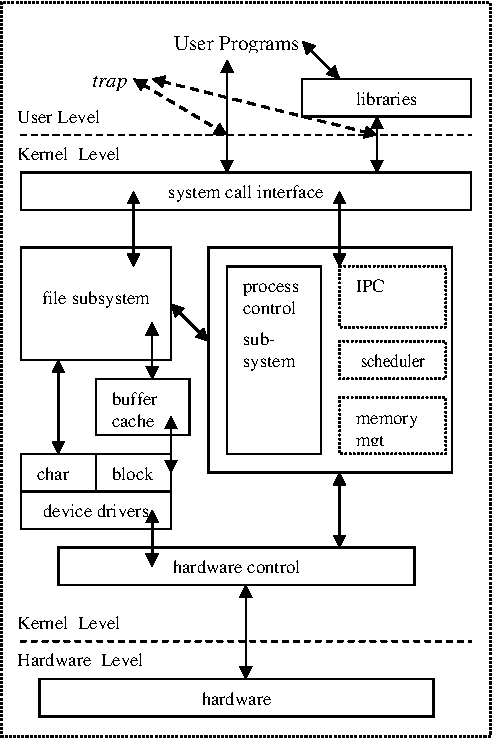
\includegraphics[width=0.52\linewidth]{fig/kernel-abstractions.pdf}
\caption{Kernel Abstractions \cite{ref7}}\label{fig:kernel}
\end{figure}


\subsection{Hierarchical File Systems
(HFS)}

Today the most common form of commercial file system is the hierarchical
structure. This model works well on several levels. For the user, it
represents a readily understood paradigm, providing an intuitive mapping
to the familiar file cabinet\(\rightarrow\)drawer\(\rightarrow\)folder\(\rightarrow\)file model prevalent in the
paper world. For the operating system it serves as a means of presenting
clumps of data as logically discrete units (files, directories, etc.).
This has the effect of simplifying both kernel and application code
while reducing the time required for operations that traverse a file
set.

\subsection{Models for Large File Dispersal using
HFS}

Recognizing that as file counts continue to grow the problem of file
location grows likewise, storage researchers have proposed a number of
models that attempt to mitigate this effect. The majority of the
proposed models create some form of central naming authority that has
jurisdiction over a domain of storage systems \cite{ref11,ref12,ref13,ref14}. The principal
strength of these models is their attempt to retain legacy HFS
semantics; predictably, this is also their most common weakness. Adding
yet another layer onto the OS/FS model necessarily adds complexity while
simultaneously increasing fragility, proving yet again the wisdom of
Occam's Razor. Further, bound by the constraint of traditional HSF
semantics such systems have difficulty achieving meaningful distinction.

While these models are ambitious in their attempt to normalize a large
namespace, they hedge on the fundamental question of who owns
responsibility for file location: the application or the file system?

Though hierarchical file systems (HFS) have proven an excellent
abstraction as a general purpose file system, further refinement is
required to address the unique operating requirements of fixed-content
data storage, retrieval, and data validation. Particularly with respect
to removing the burden from the application to meet these requirements.
